\documentclass[PROP_AGutteridge_CS.tex]{subfiles}

\begin{document}

\chapter{Related Work}
Comparable systems will be reviewed and contrasted in order to provide context to the proposed project.

\section{GoPubMed}
Developed by Michael Schroeder and colleagues at Dresden University, GoPubMed is a server and web interface that provides PubMed search results informed by the Gene Ontology database\cite{doms}. By extracting terms present in the Gene Ontology database from abstracts, GoPubMed has an improved vocabulary for genes and the gene products, enabling discovery of relevant papers that may be missed by the default PubMed search algorithm. The web interface also has additional functionality by providing shortcuts to 'Highly Related Concepts', authors and locations (Fig.1a), as well as visual representations of the data (Fig.1b) \\

\begin{figure}
	\begin{subfigure}{1\textwidth}
		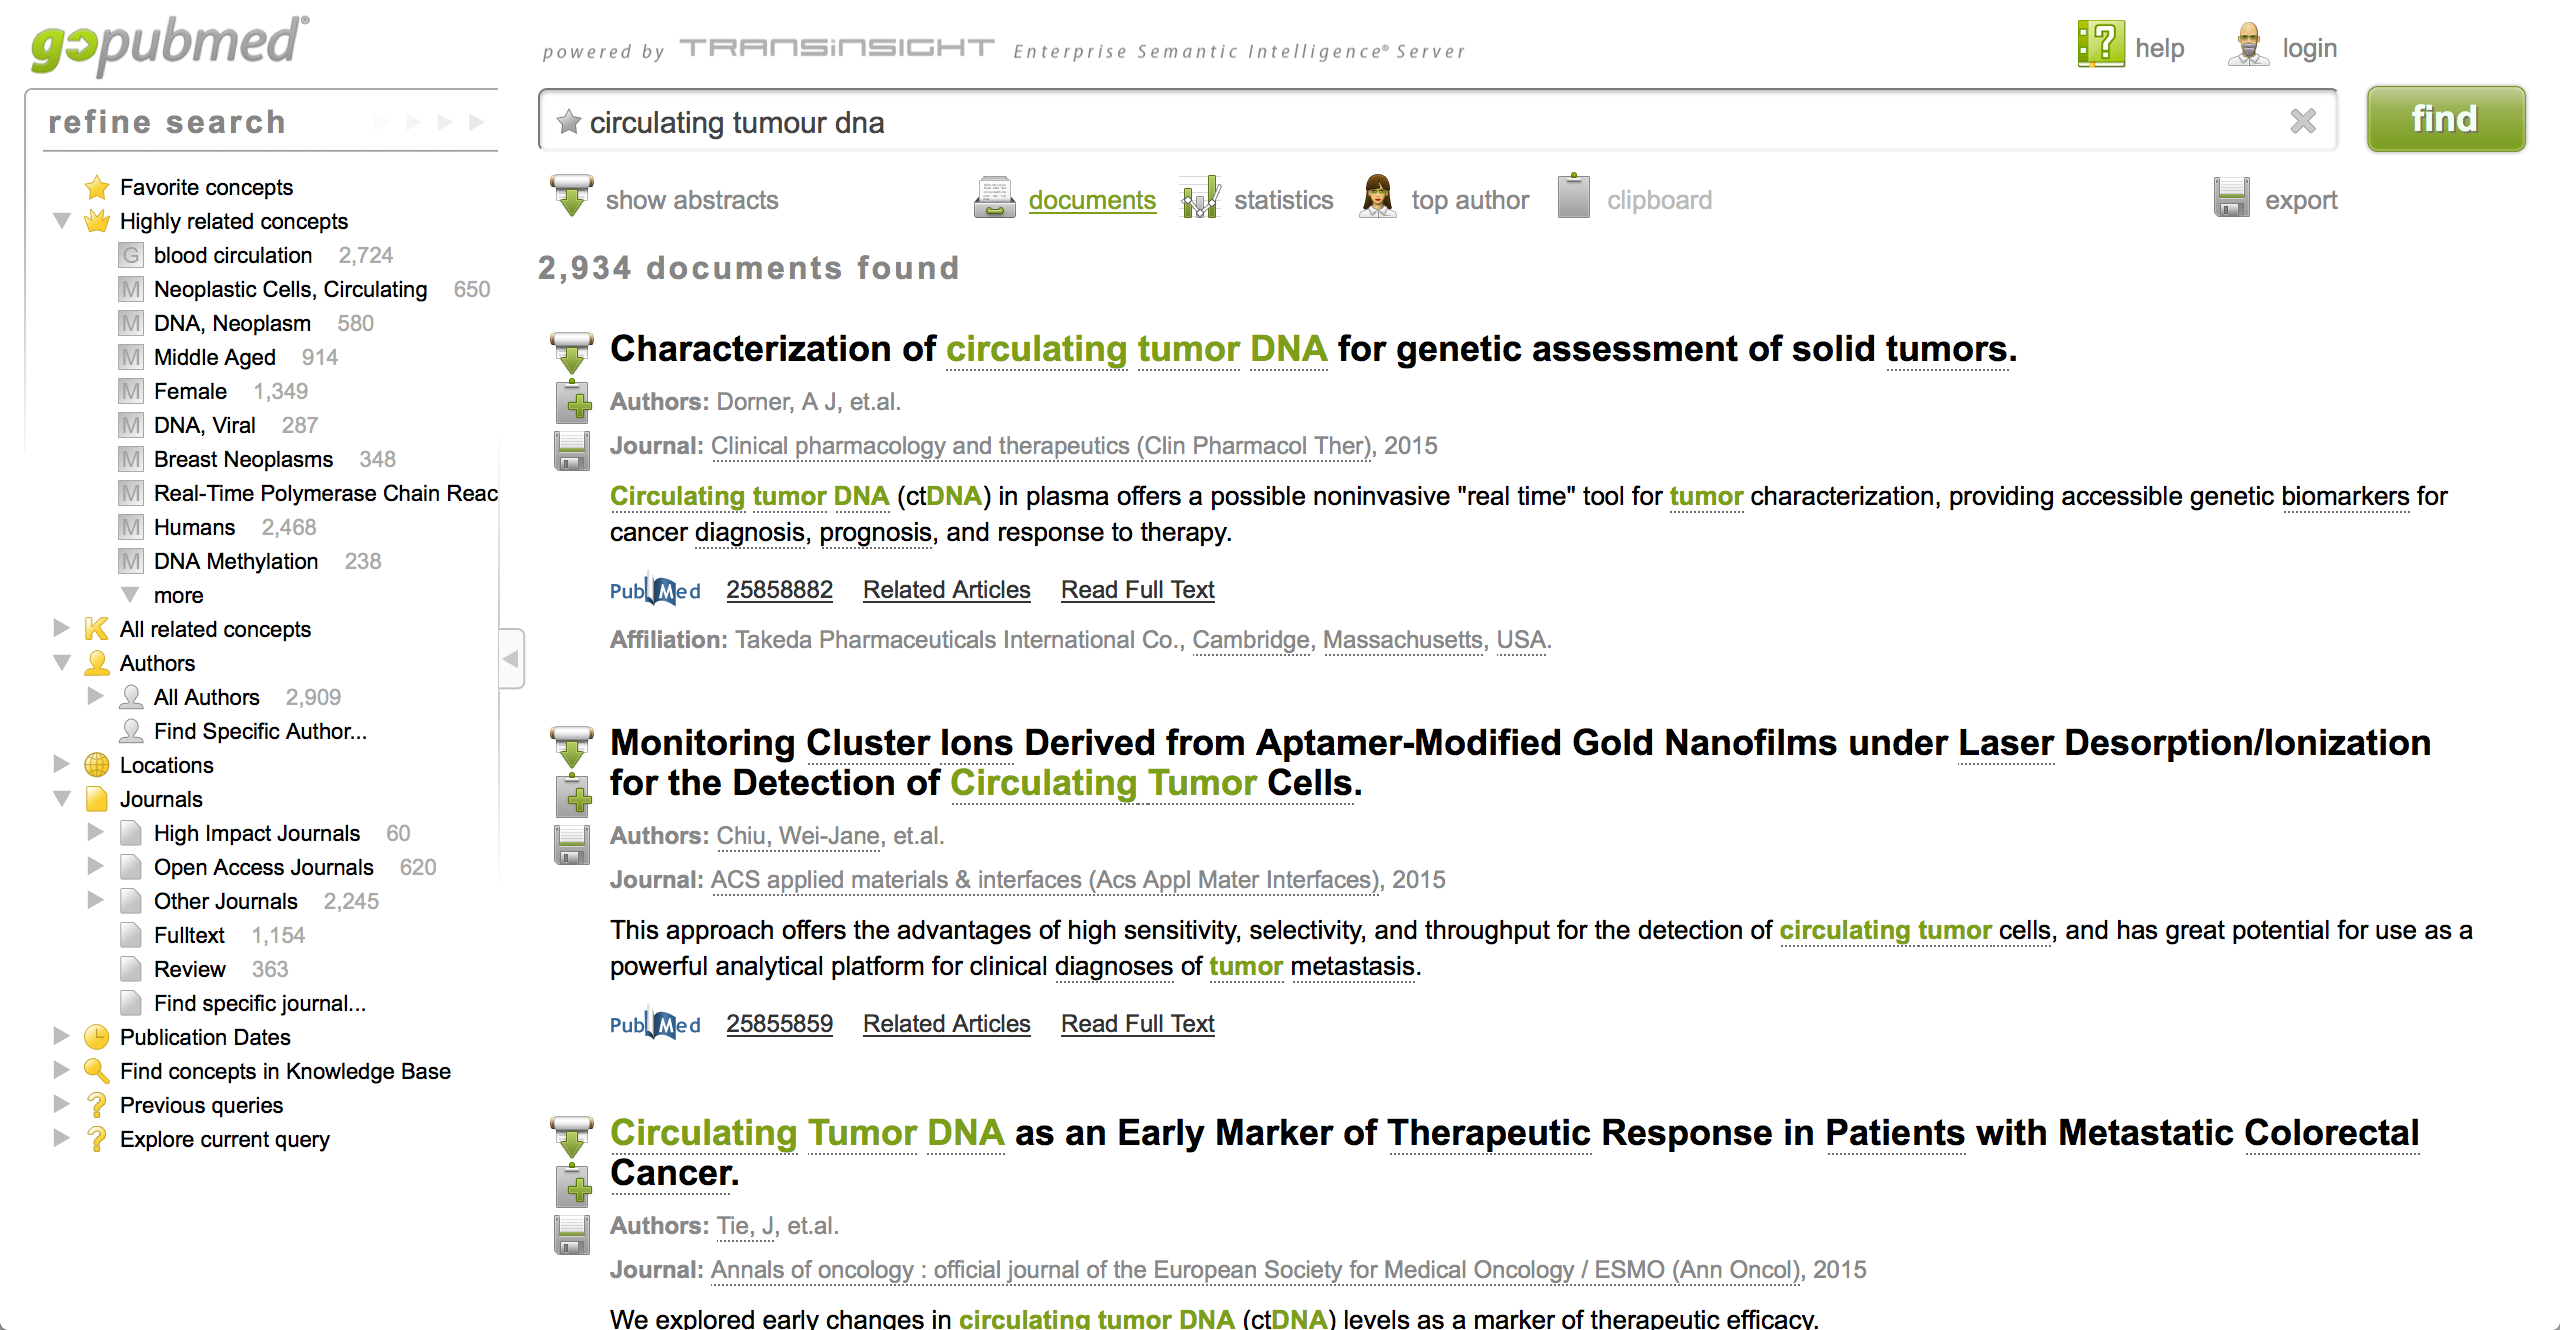
\includegraphics[width=\textwidth]{../lib/images/GPM1}
		\label{fig:GPM1}
		\subcaption{Documents view}
	\end{subfigure}\\
	\begin{subfigure}{1\textwidth}
		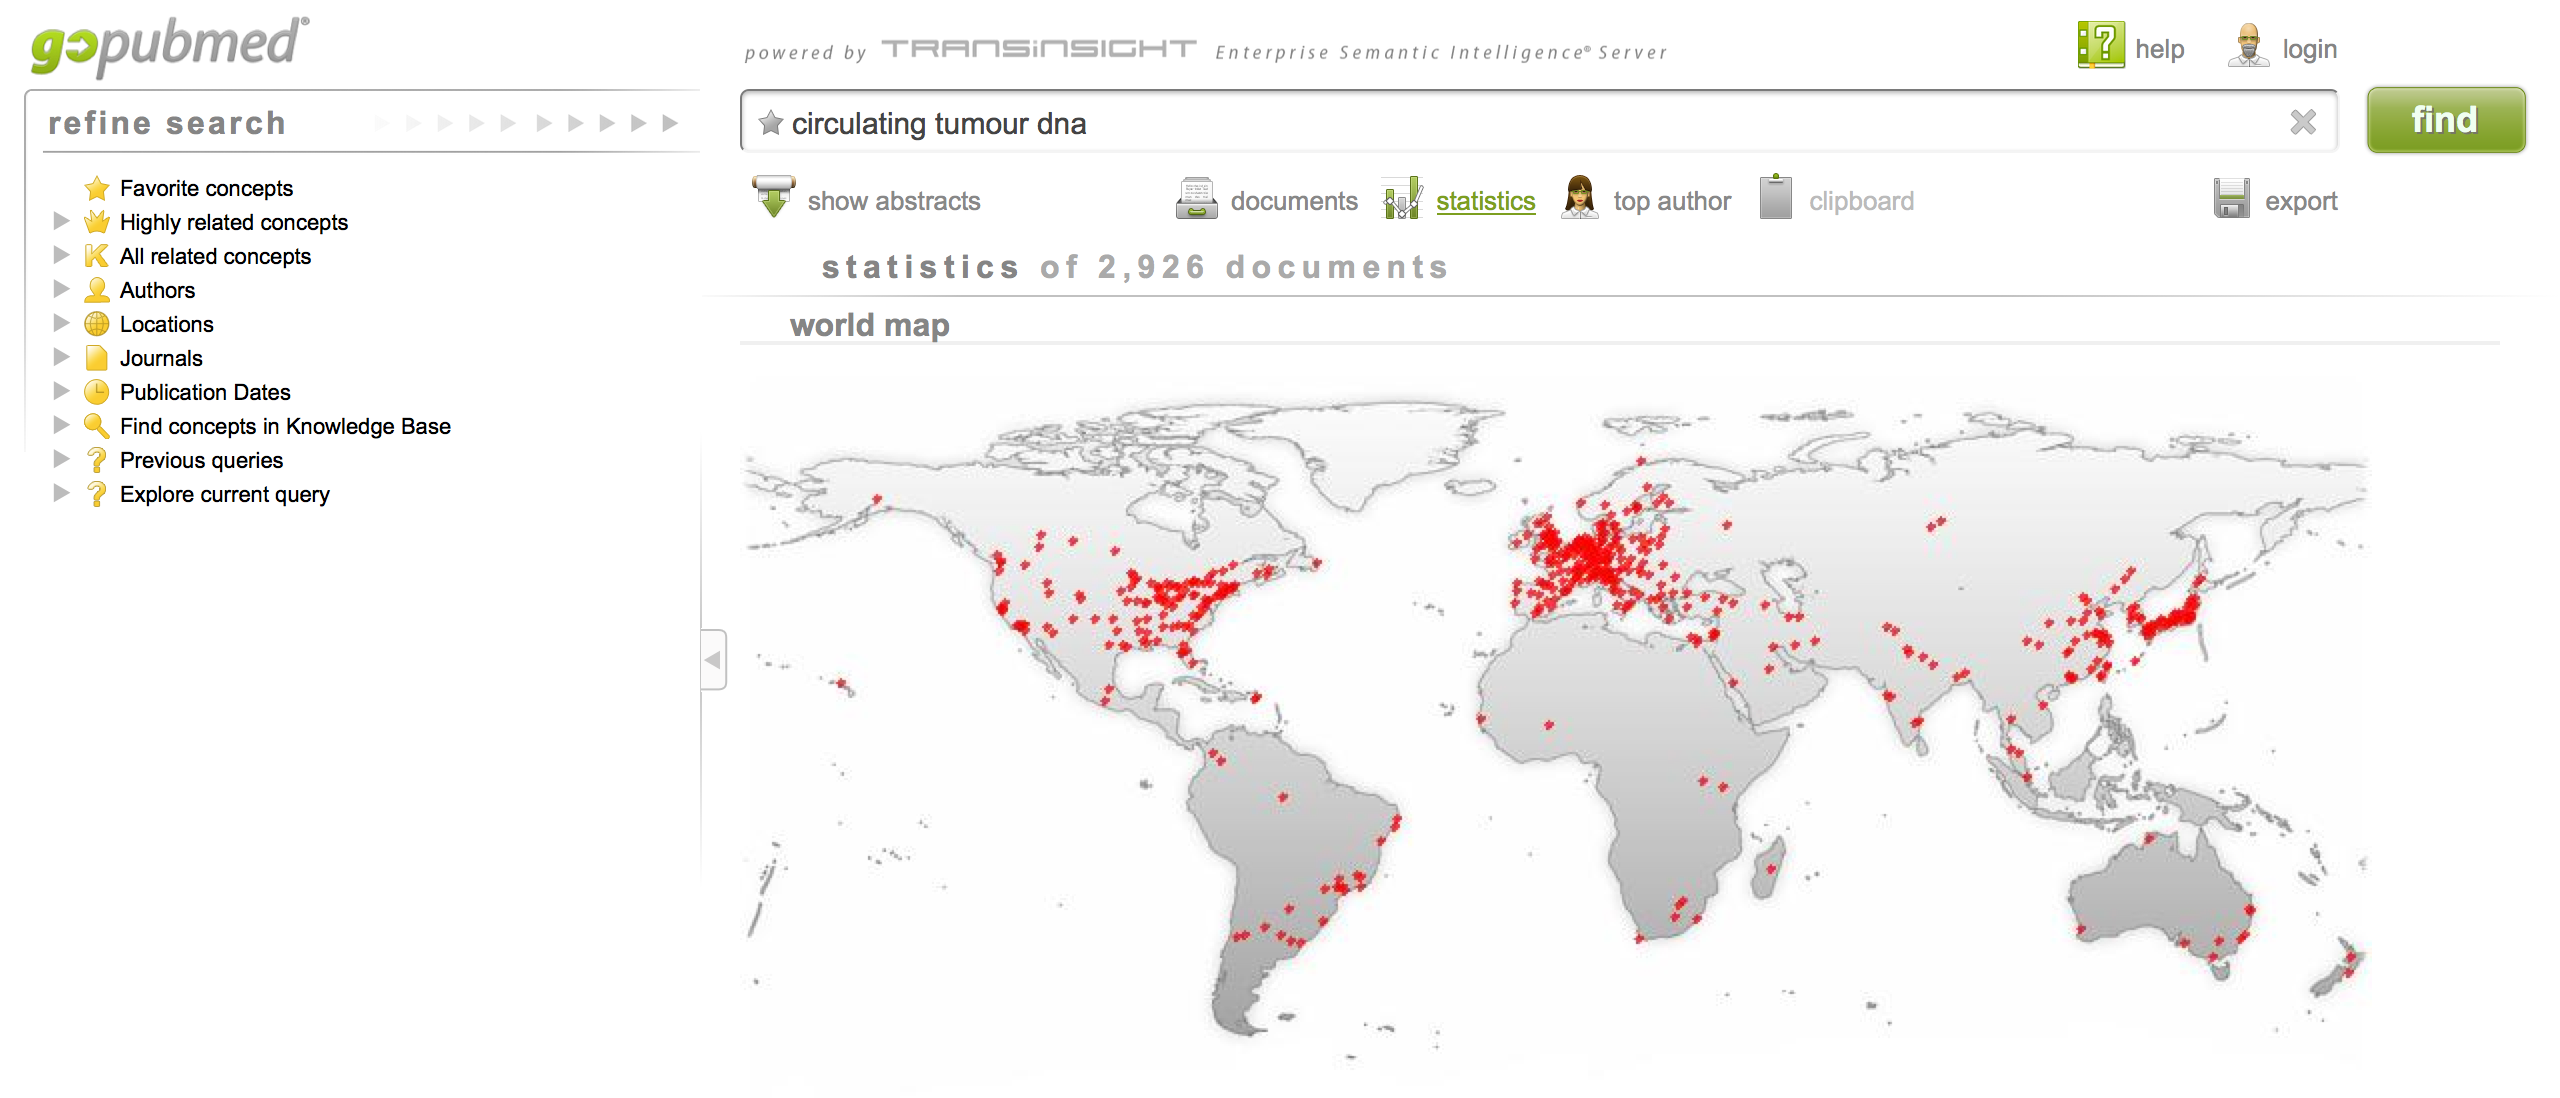
\includegraphics[width=\textwidth]{../lib/images/GPM4}
		\label{fig:GPM4}
		\subcaption{Statistics view}
	\end{subfigure} 
\caption{Web interface of GoPubMed. a) Screen after a search term has been entered. The main component of the page is the list of relevant documents, ordered by latest publication date. Additional filters are available in the sidebar to the right. b) When the 'statistics' hyperlink is followed, graphics are generated from the result data. This screenshot demonstrates a generated static JPEG showing the geographical locations of all authors.}
\end{figure}

\noindent Due to the aims of the project as described\cite{doms}, the applicability is largely limited to the field of Molecular Biology where genes and proteins are of primary interest. In the sidebar, both 'Highly Related Concepts' and 'All related Concepts' are drop-down menus providing keywords that are most prevalent in the citations retrieved by the search algorithm. I LIKE THE IDEA OF THIS as it shows research and publication trends, and may allow the user to explore different techniques, related fields or conditions. THE DOWNSIDE to the approach that GoPubMed uses is that the most common 'Highly Related Concepts' are often generic. For example, using the search term 'pancreatic cancer', the top 3 'Highly Related Concepts' are: Middle Aged, Survival, and Pancreatectomy\footnote{Query ran 07/04/15.}, arguably only the last of which could be of conducive to a user's search. Additional filters are also provided as part of the interface, allowing the user to specify, for example, that only papers authored in the United Kingdom should be shown. A map of authors is generated from all results pages (Fig.1b), the static property of which precludes direct user interaction. GoPubMed is an interesting example of extending the PubMed experience, as  Overall I feel like this website is achieving similar but not exactly what I want because it is less focused and still produces results as a textual list. I would prefer to do things dynamically as all information needed is already available in fields (don't intend to look in abstracts)

Talk about concepts that come up really high but really are not very helpful i.e. Middle-Aged, Male, Female !! Use hierarchical structure in order to filter these out?

\section{HubMed}
kind of just another interface to pubmed but provides citations. deprecated? another figure.

\section{Microsoft Academic Map}
deprecated, high level information that often navigates away to new page (based on whether academic, institution is clicked on) resolution of institutions improves as map is zoomed = good! Unable to resolve UCL, potentially due to multiple locations?

\section{Discussion}
Combination of these with emphasis on visual interface, institution locations and entity separation, organisation of MeSH keywords. OBJECTIVES.

\end{document}